% https://nymity.ch/tikz/

\documentclass[hyperref={pdfpagelabels=true},table,dvipsnames,14pt,aspectratio=169]{beamer}
\usetheme{Boadilla}
\setbeamertemplate{navigation symbols}{}

\usepackage{amsthm, amsfonts, amssymb, amsmath, graphicx}
\usepackage{amsmath}
\usepackage{mathtools}
\usepackage{amsfonts, txfonts}
\usepackage{wasysym}
\usepackage{xcolor}
\usepackage{caption}
\usepackage{comment}
\usepackage{cryptocode}
\urlstyle{same}
\usepackage{framed}
\FrameSep5pt

\usepackage{multicol}

%\usepackage[flushmargin]{footmisc}
%\setlength\footnotemargin{1em}

\usepackage{graphicx}
\graphicspath{ {images/} }

\usepackage{tikz}
\usepackage{tikzpeople}
\usepackage{pgfplots}
\usetikzlibrary{arrows}

\usetikzlibrary{positioning}
\usetikzlibrary{calc}
\usetikzlibrary{shapes}
\usetikzlibrary{shapes.callouts}

\usepackage{capt-of}
\beamertemplatenavigationsymbolsempty
\setbeamercovered{transparent}


\newcommand{\dan}[1]{ { \color{cyan}  Dan:  #1 } }
\newcommand{\chelsea}[1]{ { \color{violet}  Chelsea: #1 } }


\newcommand{\cognac}{Cognac\xspace}
\newcommand{\cognaclim}{Cognac\hbox{-}Limited\xspace}

\newcommand{\defn}[1]{{\bf {#1}}}

\newcommand\supth{\ensuremath{^{\textrm{\scriptsize th}}}}
\newcommand{\abs}[1]{\left\lvert#1\right\rvert}
\newcommand{\bigabs}[1]{\bigl| #1 \bigr|}
\newcommand{\iseq}{\stackrel{?}{=}}
\newcommand{\zo}{\{ 0, 1\}}

\newcommand{\id}{\mathsf{id}}

\newcommand{\ass}{\mathsf{assumption}}
\newcommand{\digest}{\mathsf{digest}}


% prelim
\newcommand{\MM}{\mathcal{M}}

% games
\newcommand{\BigO}{\mathcal{O}}
\newcommand{\oracle}{\BigO}
\newcommand{\G}{\mathbb{G}}
\newcommand{\GG}{\G}
\newcommand{\gpar}{\mathcal{G}}
\newcommand{\F}{\mathbb{F}}
\newcommand{\main}{\mathsc{main}}
\newcommand{\secp}{\lambda}
\newcommand{\usecp}{1^{\secp}}
\newcommand{\rgets}{\hskip2.3pt{\gets\!\!\mbox{\scriptsize${\$}$\normalsize}}\,}
\newcommand{\randpick}{\rgets}
\newcommand{\biased}{\mathsf{biased}}
\newcommand{\notbiased}{\mathsf{uniform}}
\newcommand{\random}{\rgets}
\newcommand{\pr}{\mathsf{Pr}}
\newcommand{\adv}{\mathcal{A}}
\newcommand{\negl}{\nu}
\newcommand{\advant}[2]{\ensuremath{\textsf{Adv}^{\textrm{#1}}_{#2}}}


\newcommand{\transcript}{\mathsf{trans}}
\newcommand{\nonce}{\mathsf{nonce}}
\newcommand{\session}{\mathsf{\mu}}
\newcommand{\xcoord}{\tau}

\newcommand{\Ind}{W}
\newcommand{\B}{\mathcal{B}}
\newcommand{\C}{\mathcal{C}}
\newcommand{\X}{\mathcal{X}}
\newcommand{\Sign}{\mathsf{Sign}}
\newcommand{\Hash}{\mathsf{H}}
\newcommand{\Hrho}{\mathsf{H}_{\rho}}
\newcommand{\Hcom}{\mathsf{H}_{c}}
%\newcommand{\Hpop}{\mathsf{H}_{pop}}
\newcommand{\Hblind}{\mathsf{H}_{bl}}
\newcommand{\Qrho}{\mathsf{Q}_{\rho}}
\newcommand{\Qpop}{\mathsf{Q}_{pop}}
\newcommand{\Qblind}{\mathsf{Q}_{bl}}

\newcommand{\state}{st}
\newcommand{\honest}{\mathsf{honest}}
\newcommand{\corrupt}{\mathsf{corrupt}}

% secret sharing
\newcommand{\shamir}{\mathsf{Shamir}}
\newcommand{\issueshares}{\mathsf{Share}}
\newcommand{\deterministicshare}{\mathsf{DeterministicShare}}
\newcommand{\recover}{\mathsf{Recover}}
\newcommand{\recoveryset}{\mathsf{R}}
\newcommand{\commit}{\mathsf{Commit}}
\newcommand{\verify}{\mathsf{Verify}}
\newcommand{\prove}{\mathsf{Prove}}
\newcommand{\vsscommit}{\vec{C}}
\newcommand{\vsscommitone}{\vec{D}}
\newcommand{\vsscommittwo}{\vec{E}}
\newcommand{\identifycheaters}{\mathsf{IdentifyCheaters}}

% PVPRF
\newcommand{\cvprf}{\mathsf{CVPRF}}
\newcommand{\extract}{\mathsf{Extract}}
\newcommand{\derive}{\mathsf{Derive}}
\newcommand{\witness}{\mathit{w}}
\newcommand{\commitment}{\mathit{C}}
\newcommand{\commitmenthash}{\bar{c}}
\newcommand{\blinding}{\psi}
\newcommand{\witnessspace}{\mathcal{W}}
\newcommand{\blindingspace}{\mathcal{B}}

% DKG
\newcommand{\dkg}{\mathcal{D}}
\newcommand{\keygen}{\mathsf{KeyGen}}
\newcommand{\qual}{\mathsf{qual}}

\newcommand{\polyone}{\textit{f}}
\newcommand{\polytwo}{\textit{h}}
\newcommand{\polythree}{\textit{h}'}


% algorithms
\newcommand{\Setup}{\mathsf{Setup}}
\newcommand{\ParGen}{\mathsf{Setup}}
\newcommand{\pp}{\mathsf{par}}
\newcommand{\KeyGen}{\mathsf{KeyGen}}

\newcommand{\GJKRAttack}{Key\hbox{-}Influence\xspace} % naming for GJKR attack
\newcommand{\GJKRConstruction}{GJKR\xspace} % naming for GJKR construction

\newcommand{\Z}{\mathbb{Z}}
\newcommand{\Zq}{\Z_q}
\newcommand{\Zp}{\Zq}
\newcommand{\pk}{\mathit{pk}}
\newcommand{\PK}{\pk}
\newcommand{\sk}{\mathit{sk}}
\newcommand{\SK}{\sk}
\newcommand{\secretshare}{\mathit{s}}
\newcommand{\secretshareone}{\mathit{u}}
\newcommand{\secretsharetwo}{\mathit{v}}
\newcommand{\secret}{\gammma}
\newcommand{\secretone}{\alpha}
\newcommand{\secrettwo}{\beta}
\newcommand{\blindingsum}{\phi}

% Threshold notation
\newcommand{\shareone}{\bar{u}}
\newcommand{\sharetwo}{\bar{v}}

\newcommand{\lagrange}{\lambda}
\newcommand{\DKG}{\mathsf{DKG}}
\newcommand{\SIM}{\mathsf{SIM}}
\newcommand{\simid}{\ell}

% construction two
\newcommand{\bcomm}{\delta}
\newcommand{\dkgchal}{Y}
\newcommand{\win}{y}
\newcommand{\indeter}{Z}


% games
\newcommand{\algcom}{\em\ \ /\!/ \  }

\newcommand{\Perfect}{Perfect}
\newcommand{\Bounded}{Bounded}
\newcommand{\Relative}{Relative}




% Method to add an item that will appear in every slide
%\addtobeamertemplate{footline}{%
%
%  \tikz[remember picture, overlay] \fill[blue] (current page.south east)
%    rectangle ++(1cm,2cm);
%
%}{}


\pgfdeclarelayer{background}
\pgfdeclarelayer{backbackground}
\pgfdeclarelayer{foreground}
\pgfsetlayers{backbackground,background,main,foreground}   %% some additional layers for demo

\usetikzlibrary{shapes,decorations.shapes}
\tikzset{>=latex}



\makeatletter
\pgfdeclareshape{document}{
\inheritsavedanchors[from=rectangle] % this is nearly a rectangle
\inheritanchorborder[from=rectangle]
\inheritanchor[from=rectangle]{center}
\inheritanchor[from=rectangle]{north}
\inheritanchor[from=rectangle]{south}
\inheritanchor[from=rectangle]{west}
\inheritanchor[from=rectangle]{east}
% ... and possibly more
\backgroundpath{% this is new
% store lower right in xa/ya and upper right in xb/yb
\southwest \pgf@xa=\pgf@x \pgf@ya=\pgf@y
\northeast \pgf@xb=\pgf@x \pgf@yb=\pgf@y
% compute corner of ‘‘flipped page’’
\pgf@xc=\pgf@xb \advance\pgf@xc by-10pt % this should be a parameter
\pgf@yc=\pgf@yb \advance\pgf@yc by-10pt
% construct main path
\pgfpathmoveto{\pgfpoint{\pgf@xa}{\pgf@ya}}
\pgfpathlineto{\pgfpoint{\pgf@xa}{\pgf@yb}}
\pgfpathlineto{\pgfpoint{\pgf@xc}{\pgf@yb}}
\pgfpathlineto{\pgfpoint{\pgf@xb}{\pgf@yc}}
\pgfpathlineto{\pgfpoint{\pgf@xb}{\pgf@ya}}
\pgfpathclose
% add little corner
\pgfpathmoveto{\pgfpoint{\pgf@xc}{\pgf@yb}}
\pgfpathlineto{\pgfpoint{\pgf@xc}{\pgf@yc}}
\pgfpathlineto{\pgfpoint{\pgf@xb}{\pgf@yc}}
\pgfpathlineto{\pgfpoint{\pgf@xc}{\pgf@yc}}
}
}
\makeatother


\usepackage{filecontents}

\begin{filecontents}{msr-start.bib}



\end{filecontents}




\title{Attacks and Fixes on Distributed~Key~Generation~Protocols}
\author{Chelsea Komlo, University of Waterloo}
\date[November 2021]{ Cryptography Reading Group, November 2021}

\begin{document}
\setbeamertemplate{itemize items}[triangle]

\tikzstyle{doc}=[%
draw,
thick,
align=center,
color=black,
shape=document,
minimum width=12mm,
minimum height=15.2mm,
shape=document,
inner sep=2ex,
]

\begin{frame}
        \thispagestyle{empty}
        \maketitle
\end{frame}


\begin{frame}
  \frametitle{Distributed Key Generation (informal)}

  \begin{itemize}
    \item<1-> Generating key material without relying on a trusted entity is often desirable for distributed protocols.
    \item[]
    \item<2-> In a DKG, $n$ parties (chosen beforehand) participate, all equally trusted.
    \item[]
    \item<3-> Goal is to:
  \begin{itemize}
    \item<4-> Generate a secret that all parties contribute to but no party knows
    \item<5-> $t$ parties are required to recover.
    \item<6-> While $t$ can equal $n$, the setting where $t \leq n$ is often desirable.
  \end{itemize}
    %\item[]
    %\item<6-> A common mechanism is to perform $n$-wise secret sharing with an aggregation step at the end (more on this later).
  \end{itemize}
\end{frame}

\begin{frame}
  \frametitle{DKG Threat Model}

  \begin{itemize}
    \item<1-> At minimum, requires assuming the adversary can control up to $t-1$ players.
    \item[]
    \item<2-> If the adversary controlled $t$ players, they could trivially recover the secret.
  \end{itemize}
\end{frame}

\begin{frame}
  \frametitle{Use Cases for DKGs}

  \begin{itemize}
    \item<1-> Key generation for threshold or multiparty signatures
    \item[]
    \item<2-> Distributed PRFs (League of Entropy)
    \item[]
    \item<3-> Key generation for anonymous token issuance (Privacy Pass)
  \end{itemize}
\end{frame}


\begin{frame}
  \frametitle{A Trivial $n$-out-of-$n$ DKG}

  \begin{itemize}
    \item<1-> Each party $i$ begins by:

  \begin{itemize}
    \item<2-> Sampling $x_i \rgets \Zq$
    \item<3-> Generating $X_i \gets g^x$
    \item<4-> Generating the commitment $c_i \gets H(X_i)$
    \item<5-> Each party publishes their commitment to all other parties.
  \end{itemize}
    \item[]
    \item<6-> After having received all $c_1, \ldots, c_n$, each party publishes $X_i$
    \item<7-> Each party checks that $c_i \iseq H(X_i)$. If not, they abort and identify misbehaving parties.
    \item<8-> Otherwise:
  \begin{itemize}
    \item<9-> $\pk \gets \prod X_i$
    \item<10-> While unknown to any party, $\sk \gets \sum x_i$
  \end{itemize}

  \end{itemize}
\end{frame}

\begin{frame}
  \frametitle{$t$-out-of-$n$ DKGs}

  \begin{itemize}
    \item In practice, it is desirable to require only a \emph{subset} of the parties to be online.
    \item[]
    \item<2-> For example, secret keys may be lost or a server might be unavailable.
    \item[]
    \item<3-> $t$ is referred to as the \emph{threshold} number of participants required to participate.
    \item[]
    \item<4-> $n$ is the total number of participants.
  \end{itemize}
\end{frame}


\begin{frame}
  \huge
  \centering
  Background
\end{frame}

\begin{frame}
  \frametitle{Shamir Secret Sharing}

  \begin{itemize}
    \item<1-> Allows a \emph{dealer} to share a secret $\secretone$ among $n$ participants, where $t$ participants must cooperate to recover $\secretone$.
    \item<2-> $f$ is the polynomial defined by the coefficients

      \[f = \secretone + a_1 x + a_2 x^2 + a_3 x^3 + \ldots + a_{t-1}x^{t-1}  \]

    \item<3-> Each participant $i \in \{1, \ldots, n \}$ receives a share $\shareone_i \gets f(i) $.
    \item<4-> Recall that $t$ points uniquely define a polynomial of degree $t-1$!
    \item<5-> By polynomial interpolation, $\secretone = f(0) = \sum_{i=1}^t f(i) \lambda_i$.
    \item<6-> $\lambda_i$ is $L_i(0)$, where $L_i$ is the $i\supth$ Lagrange polynomial for the set $\{1, \ldots, t \}$.
  \end{itemize}
\end{frame}

\begin{frame}
  \frametitle{Verifiable Secret Sharing}

  \begin{itemize}
    \item<1-> Allows participants to verify their share $\shareone_i = f(i)$ is on the same polynomial as all other participants,
      \emph{without} revealing $f$ directly.
    \item[]
    \item<2-> Working in the discrete log setting: a commitment to $f$ is $\vsscommitone \gets \langle A_0, A_1, \ldots, A_{t-1}  \rangle$, where

      \[ A_0 \gets g^{\secretone},\ A_1 \gets g^{a_1}, \ldots \]
    \item[]
    \item<3-> Verification of shares requires performing polynomial interpolation in the exponent to check that $g^{f(i)}$ is a point on $g^f$.
  \end{itemize}
\end{frame}

\begin{frame}
  \frametitle{Rushing Adversary}

  \begin{itemize}
    \item<1-> In a multi-party protocol where scheduling of communication is not enforced, an adversary can choose when to participate.
    \item[]
    \item<2-> A \emph{rushing adversary} is one that waits to ``speak last'', and so learns every other participant's contributions before selecting their own.
  \end{itemize}
\end{frame}

\begin{frame}
  \huge
  \centering
  Distributed Key Generation
\end{frame}

\begin{frame}
  \frametitle{DKG Definition}

  A DKG is the tuple $(\keygen, \recover)$, such that:

  \begin{itemize}
    \item<2-> $\mathit{KeyGen}(\lambda, n, t) \rightarrow ( \pk, \qual, \{\sk_1, \ldots, \sk_n \} )$
    \begin{itemize}
      \item<3-> A probabilistic protocol among $n$ predetermined parties.
      \item<4-> Output to each party includes:
    \begin{enumerate}
      \item<5->[1.] Public key $\pk$
      \item<6->[2.] The set $\qual$ of parties remaining at the end.
      \item<7->[3.] Their secret key share $\sk_i$.
    \end{enumerate}

    \item<8-> Importantly:

    \end{itemize}
    \item[]
    \item<8-> $\mathit{Recover}(\{ \sk_i \}_C) \rightarrow \sk$
    \begin{itemize}
      \item<9-> A deterministic algorithm performed by one entity.
      \item<10-> Assuming $\lvert C \rvert \geq t$, $\sk$ is recovered by combining $\{ \sk_i \}_C$.
    \end{itemize}
  \end{itemize}
\end{frame}

\begin{frame}
  \frametitle{On Determining $\qual$}

  \begin{itemize}
    \item<1-> Because cheating parties can be picked out during protocol execution,
      \[ t \leq \lvert \qual \rvert \leq n \]
    \item[]
    \item<2-> If $\qual \not\geq t$, then the DKG simply fails, as $t$ parties are required for $\mathit{Recover}$.
    \item[]
    \item<3-> Parties perform a sub-protocol to identify and kick out cheaters.
  \end{itemize}
\end{frame}

\begin{frame}
  \frametitle{Correctness of a DKG}

  \begin{itemize}
    \item<1-> All subsets of $t$ shares define the same secret key $\sk$ (or any subset fulfilling the required access structure)
\let\thefootnote\relax\footnote{
Gennaro, Rosario and Jarecki, Stanislaw and Krawczyk, Hugo and Rabin, Tal. Secure Distributed Key Generation for Discrete-Log Based Cryptosystems. Journal of Cryptology, 2007
}
    \item[]
    \item<2-> All parties that honestly followed the protocol have the same value of the public key $\pk$.
  \end{itemize}
\end{frame}

\begin{frame}
  \frametitle{Security: Two Approaches}

  \begin{itemize}
    \item<1-> \emph{Stand-Alone}: The DKG can be proven secure without reference to how it is used.
    \begin{itemize}
      \item<2-> Nothing about $\sk$ is revealed beyond what is revealed by $\pk$ (from GJKR).
      \item<3-> The protocol can be perfectly simulated to an adversary for a challenge public key.
      \item<4-> In other words, the simulated DKG must output the challenge as the group's public key.
    \end{itemize}

    \item[]
    \item<5-> \emph{Contextual}: Prove the security of the DKG in the context of demonstrating security of the protocol in which it is used
  \footnote{
  Kobi Gurkan, Philipp Jovanovic, Mary Maller, Sarah Meiklejohn, Gilad Stern, Alin Tomescu.
  Aggregatable Distributed Key Generation, EUROCRYPT 2021 }
  \end{itemize}
\end{frame}

\begin{frame}
  \frametitle{Security: Two Approaches (cont'd)}

  \begin{itemize}
    \item<1-> \emph{Stand-Alone}:
  \begin{itemize}
    \item<2-> Pro: Proving security means that the DKG can be used in any context.
    \item<3-> Con: Very hard definition to achieve, requires guaranteed output delivery.
  \begin{itemize}
    \item<4-> No notion of failure and/or rewinding in the existing definition.
    \end{itemize}
    \end{itemize}
    \item[]
    \item<5-> \emph{Contextual}:
  \begin{itemize}
    \item<6-> Pro: Allows for more efficient protocols to be proven secure (more on this later).
    \item<7-> Con: Proofs are unwieldy and requires proving the security of the DKG over and over in different use cases.
    \end{itemize}
  \end{itemize}
\end{frame}

\begin{frame}
  \frametitle{Requirement of Security: Uniform Distribution}

  \begin{itemize}
    \item<1-> In a single-party setting, ensuring that a secret key is randomly sampled is easy.
    \item[]
    \item<2-> In a multi-party setting, where the adversary is a participant,
      ensuring key material is uniformly distributed is harder.
    \item[]
    \item<3-> For example: $\gamma \gets \alpha + \sum_{i=1}^n \beta_i$
  \begin{itemize}
    \item<4-> Here, $\alpha \rgets \Zq$ and each $b_i$ is chosen non-uniformly.
    \item[]
    \item<5-> $\gamma$ is random if each $\beta_i \in \Zq$ is chosen \emph{without} knowledge of $\alpha$.
    \item[]
    \item<6-> Otherwise, $\gamma$ is not random.
  \end{itemize}
  \end{itemize}
\end{frame}

\begin{frame}
  \huge
  \centering
  Current Landscape
\end{frame}

\begin{frame}
  \frametitle{Pedersen DKG: Overview}

  \begin{itemize}
    \item<1-> Each participant $i$ acts as the dealer and performs a Shamir secret sharing of a secret $\secretone_i$,
      distributing shares $\shareone_{ij}$ to each other.
    \item[]
    \item<2-> The group's secret at the end is $\sk \gets \sum \secretone_i = \sum \sum \shareone_{ij} \lambda_i$.
    \item[]
    \item<3-> Proven secure in the context of threshold signatures.
  \footnote{
  Rosario Gennaro, Stanislaw Jarecki, Hugo Krawczyk, Tal Rabin.
  Secure Applications of Pedersen's Distributed Key Generation Protocol,
  CT-RSA, 2003.}
    \item[]
    \item<4-> A rushing adversary \emph{can} bias key material, but by a limited amount.
  \end{itemize}
\end{frame}




\begin{frame}
  \centering
\begin{tikzpicture}
\node at (0,0) {
\scalebox{0.9} {
  \procedure{Pedersen DKG}{
  \textbf{Participant i}  \> \textbf{Other Participants}  \\
  \uncover<1-> { \secretone_i  \rgets \Zq \\ }
  \uncover<2-> { (\{ \shareone_{i1}, \ldots, \shareone_{in}\}, \{\secretone_i, a_{i1}, \ldots, a_{i(t-1)} \}) \rgets \shamir.\issueshares(\secretone_i, n, t) \> \\ }
  \uncover<3-> { \vsscommitone_i  = \langle A_{i0}, \ldots, A_{i(t-1)} \rangle \gets \shamir.\commit(\secretone_i, a_{i1}, \ldots, a_{i(t-1)}) \> \\ }
  \uncover<4-> { \> \sendmessageright{top=\text{ {\bf Broadcast}  $\vsscommitone_i $   }}  \< \\}
  \uncover<5-> { \> \sendmessageright{top=\text{ {\bf Send} $\shareone_{ij} $   }}  \< \\ }
  \uncover<6-> {  \shamir.\verify(\shareone_i, \vsscommitone_j) \iseq 1  \> \\ }
  \uncover<7-> { \sk_i = \sum_{k \in \qual} \shareone_k \lambda_k,\ \ \text{\algcom $\qual$ are the players that issued valid shares. }    \\ }
  \uncover<8-> {  \pk \gets  \prod_{k \in \qual} A_{k0}  = g^{\sum_{i \in \qual} \secretone_i  }   \> \\ }
}
}
};
\end{tikzpicture}
\end{frame}

\begin{frame}
  \frametitle{Key Bias Attack Against Pedersen DKG}

  \begin{itemize}
    \item<1-> A rushing adversary can learn the output public key before publishing their own contribution.
    \item[]
    \item<2-> Nothing prevents this adversary from adaptively choosing their contributions.
    \item[]
    \item<3-> We show an example of this adversary forcing $\pk$ to be even without detection from other participants.
  \end{itemize}
\end{frame}

\begin{frame}
  \centering
\begin{tikzpicture}
\node at (0,0) {
\scalebox{0.9} {
  \procedure{Key Bias Attack by a Rushing Adversary}{
  \textbf{Adversary}  \> \textbf{Other Participants}  \\
  \uncover<1-> { \> \sendmessageleft{top=\text{ {\bf Broadcast}  $\vsscommitone_i$   }}   \\}
  \uncover<2-> { \> \sendmessageleft{top=\text{ {\bf Send} $\shareone_{ij}$   }}   \\ }
  \uncover<3-> { \text{Until $\pk$ is even, do:}   } \\
  \uncover<4-> { \ \ \ \ \ \ \secretone_A  \rgets \Zq;\ \text{ check }  \pk = g^{\secretone_A} \cdot  \prod_{k =1; k \neq A}^n A_{k0}    \\ }
  \uncover<5-> { (\{ \shareone_{A1}, \ldots, \shareone_{An}\}, \{\secretone_A, a_{A1}, \ldots, a_{A(t-1)} \}) \rgets \shamir.\issueshares(\secretone_A, n, t) \> \\ }
  \uncover<6-> { \vsscommitone_A  = \langle A_{A0}, \ldots, A_{A(t-1)} \rangle \gets \shamir.\commit(\secretone_A, a_{A1}, \ldots, a_{A(t-1)}) \> \\ }
  \uncover<7-> { \> \sendmessageright{top=\text{ {\bf Broadcast}  $\vsscommitone_A $   }}  \< \\}
  \uncover<8-> { \> \sendmessageright{top=\text{ {\bf Send} $\shareone_{Aj} $   }}  \< \\ }
}
}
};
\end{tikzpicture}
\end{frame}


\begin{frame}
  \frametitle{GJKR: Overview}

  \begin{itemize}
    \item Stand-alone security; secure against key biasing.
    \item[]
    \item<2-> Assumes $t$ honest players.
    \item[]
    \item<3-> Participants issue a blinded VSS commitment in round one and then unblinds in round three.
    \item[]
    \item<4-> Share correctness is verified using blinded commitments.
    \item[]
    \item<5-> Contributions from cheating players can be extracted in round three (by $t$ honest players).
  \end{itemize}
\end{frame}

\begin{frame}
  \centering
\begin{tikzpicture}
\node at (0,0) {
\scalebox{0.9} {
  \procedure{GJKR Construction: Rounds One and Two}{
    \textbf{\underline{Participant i}}  \qquad \qquad \qquad \qquad \qquad \qquad \qquad \qquad \qquad \qquad \qquad \textbf{\underline{Other Participants}}  \\
  \uncover<1-> { \secretone_i, b_i  \rgets \Zq \\ }
  \uncover<2-> { (\{ \shareone_{i1}, \ldots, \shareone_{in}\}, \{\secretone_i, a_{i1}, \ldots, a_{i(t-1)} \}) \rgets \shamir.\issueshares(\secretone_i, n, t)  \\[1mm] }
  \uncover<3-> { \vsscommitone_i  = \langle A_{i0}, \ldots, A_{i(t-1)} \rangle \gets \shamir.\commit(g, \secretone_i, a_{i1}, \ldots, a_{i(t-1)}) \\ \qquad \qquad \text{\algcom Commit with base $g$}  \\ }
  \uncover<4-> { (\{ \sharetwo_{i1}, \ldots, \sharetwo_{in}\}, \{b_i, \hat{a_{i1}}, \ldots, \hat{a_{i(t-1)}} \}) \rgets \shamir.\issueshares(b_i, n, t)  \\[1mm] }
  \uncover<5-> { \vsscommittwo_i  = \langle \hat{A}_{i0}, \ldots, \hat{A}_{i(t-1)} \rangle \gets \shamir.\commit(h, b_i, \hat{a_{i1}}, \ldots, \hat{a_{i(t-1)}}) \\ \qquad \qquad \text{\algcom Commit with base $h$}  \\[1mm] }
  \uncover<6-> { \vsscommitthree_i  \gets \langle (A_{i0}\hat{A}_{i0}),  \ldots,  (A_{i(t-1)}\hat{A}_{i(t-1)}) \rangle   \text{\algcom Pedersen commitment }  \\[1mm] }
%
  \uncover<7-> { \qquad \qquad \qquad \qquad \qquad \qquad \sendmessageright{top=\text{ {\bf Broadcast}  $\vsscommitthree_i $   }}  \< \\[1mm] }
  \uncover<8-> { \qquad \qquad \qquad \qquad \qquad \qquad  \sendmessageright{top=\text{ {\bf Send} $\shareone_{ij},  \sharetwo_{ij}$ to player $j$   }}  \< \\ }
  \uncover<9-> { \text{If } \shamir.\verify(\shareone_{ji}, \sharetwo_{ji}, \vsscommitthree_k) \neq 1:\ \text{Identify cheaters. Otherwise:}\ \qual \gets \qual\ \bigcup\ \{i\};  \> \\ }
}
}
};
\end{tikzpicture}
\end{frame}


\begin{frame}
  \centering
\begin{tikzpicture}
\node at (0,0) {
\scalebox{0.9} {
  \procedure{GJKR Construction: Round Three}{
    \textbf{\underline{Participant i}}  \> \textbf{\underline{Other Participants}}  \\
  \uncover<1-> { \qquad \qquad \qquad \sendmessageright{top=\text{ {\bf Broadcast}  $\vsscommitone_i $   }}  \< \\[2ex]}
  \uncover<2-> { \excluded \gets \emptyset \> \\[1ex] }
  \uncover<3-> { \text{For all $j$ where } \shamir.\verify(\shareone_{ji}, \vsscommitone_j) \neq 1:  \> \\[2ex] }
  \uncover<4-> { \qquad \qquad  \excluded \gets \excluded \cup \{ j \}   \> \\[2ex] }
%
  \uncover<5-> { \sk_i = \sum_{j \in \excluded} \secretone + \sum_{k \in ( \qual \setminus \excluded)} \shareone_k \lambda_k     \\[2ex] }
  \uncover<6-> {  \pk \gets  \prod_{k \in \qual} A_{k0}  = g^{\sum_{i \in \qual} \secretone_i  }    \> \\[2ex] }
}
}
};
\end{tikzpicture}
\end{frame}


\begin{frame}
  \frametitle{Uniform Distribution of Key Material in GJKR}

  \begin{itemize}
    \item Cheating parties must choose their contributions having seen only the blinded commitment $\vsscommitthree_i$ from other players.
    \item[]
    \item<2-> Pedersen commitments guarantee that $H_i = g^ih^j$ will not reveal any information about $g^i$.
    \item[]
    \item<3-> If player $A$ cheats and is kicked out in round $3$,  $\secretone_A$ can be extracted (assuming $t$ honest parties).
    \item[]
    \item<4-> So key material will remain unbiased even if a player cheats in the last round after learning $\pk$.
  \end{itemize}
\end{frame}

\begin{frame}
  \frametitle{Proof Sketch}

  \begin{itemize}
    \item Input challenge $\dkgchal$, environment must output $\pk = \dkgchal$ while perfectly simulating the protocol.
    \item<2-> Adversary controls the set $\corrupt$, where $\lvert \corrupt \rvert \leq t-1$;
    \item<3-> Environment simulates the set $\honest$, where $\lvert \honest \rvert \geq t$.
    \item<4-> The environment follows round one and two honestly for all simulated partiest.
    \item<5-> After receiving the adversary's contributions, the environment can derive $\secretone_i, i \in \corrupt$ (as it controls $t$ parties).
  \end{itemize}
\end{frame}


\begin{frame}
  \frametitle{Proof Sketch (cont'd)}

  \begin{itemize}
    \item In round three, for one honest party $\ell$:
  \begin{itemize}
    \item<2-> Derive the commitment to the constant term relative to the adversary's secrets:

      \[ A_{\ell 0} \gets \dkgchal \cdot g^{- \sum \secretone_i},\ i \in \honest \cup \corrupt \setminus \{ \ell\}  \]

      Ensuring that:

      \[ \pk = \prod A_{i0} = \dkgchal \cdot g^{\sum a_i0 - \sum a_i0}  = \dkgchal  \]

    \item<3-> Derive all other commitments using shares published in round one
      \[ A_{\ell i} \gets  A_{\ell 0}^{\lambda_{\ell 0}} \cdot \prod g^{\shareone_{\ell j}\lambda_{\ell j }}   \]

      ensuring the VSS check holds.

  \end{itemize}
  \end{itemize}
\end{frame}

\begin{frame}
  \frametitle{Ongoing Research}

  \begin{itemize}
    \item GJKR protects key-bias attacks, but requires an additional network round.
    \item[]
    \item<2-> Goal: a two-round DKG whose security is proven in a stand-alone manner.
    \item[]
    \item<3-> This is our ongoing work; stay tuned!
  \end{itemize}
\end{frame}


\begin{frame}
  \frametitle{Takeaways}

  \begin{itemize}
    \item DKGs are a useful building block for distributing trust among set of parties.
    \item<2-> Properties for centralized protocols are difficult to guarantee in a multi-party setting (such as uniform distribution of key material).
    \item<3-> Pedersen DKG is simple and efficient, but must be proven seperately for each context which it is used.
    \item<4-> GJKR is proven in a stand-alone manner, but at the loss of efficiency.
    \item<5-> Our work achieves the best of both worlds; more to come soon!
  \end{itemize}
\end{frame}

\begin{frame}

  \huge
  \centering
  Thank you!
\end{frame}

\end{document}



\begin{frame}
  \centering
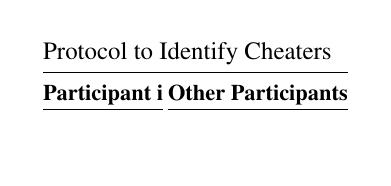
\begin{tikzpicture}
\node at (0,0) {
\scalebox{0.9} {
  \procedure{Protocol to Identify Cheaters}{
    \textbf{\underline{Participant i}}  \> \textbf{\underline{Other Participants}}  \\
}
}
};
\end{tikzpicture}
\end{frame}

